\documentclass[aspectratio=169,10pt]{beamer}

% Encoding
\usepackage[utf8]{inputenc}
\usepackage[T1]{fontenc}

% Theme — clean, minimal
\usetheme{Madrid}
\usecolortheme{seahorse}
\setbeamertemplate{navigation symbols}{}
\setbeamertemplate{footline}[frame number]

% Math
\usepackage{amsmath, amssymb, amsfonts, mathtools}
\usepackage{bm}

% Tables
\usepackage{booktabs}
\usepackage{array}
\usepackage{colortbl}

% Graphics
\usepackage{graphicx}
\usepackage{tikz}
\usetikzlibrary{arrows.meta, positioning, calc, shapes.geometric, fit, backgrounds, decorations.pathreplacing}

% Colors — dark teal academic palette
\definecolor{deepblue}{RGB}{0, 60, 113}
\definecolor{tealdark}{RGB}{0, 100, 120}
\definecolor{tealaccent}{RGB}{0, 150, 136}
\definecolor{coralaccent}{RGB}{231, 76, 60}
\definecolor{goldaccent}{RGB}{241, 196, 15}
\definecolor{lightgray}{RGB}{245, 245, 245}
\definecolor{mathbg}{RGB}{240, 248, 255}
\definecolor{codebg}{RGB}{248, 248, 248}
\definecolor{newgreen}{RGB}{39, 174, 96}

% Code
\usepackage{listings}
\lstset{
  basicstyle=\ttfamily\tiny,
  keywordstyle=\color{tealdark}\bfseries,
  commentstyle=\color{gray},
  stringstyle=\color{coralaccent},
  breaklines=true,
  frame=single,
  rulecolor=\color{lightgray},
  backgroundcolor=\color{codebg},
  showstringspaces=false,
  xleftmargin=2pt,
  xrightmargin=2pt,
  aboveskip=3pt,
  belowskip=3pt,
}

\lstdefinelanguage{bash}{
  morekeywords={segger,pip,install,export,segment,hpo,pytest},
  sensitive=true,
  morecomment=[l]{\#},
  morestring=[b]",
  morestring=[b]',
}

\setbeamercolor{frametitle}{bg=deepblue, fg=white}
\setbeamercolor{progress bar}{fg=tealaccent}
\setbeamercolor{title separator}{fg=tealaccent}
\setbeamercolor{alerted text}{fg=coralaccent}
\setbeamercolor{block title}{bg=tealdark, fg=white}
\setbeamercolor{block body}{bg=lightgray}
\setbeamercolor{block title alerted}{bg=coralaccent, fg=white}
\setbeamercolor{block body alerted}{bg=coralaccent!10}
\setbeamercolor{block title example}{bg=newgreen!80!black, fg=white}
\setbeamercolor{block body example}{bg=newgreen!5}

% Custom commands
\newcommand{\vect}[1]{\boldsymbol{#1}}
\newcommand{\mat}[1]{\mathbf{#1}}
\newcommand{\graph}{\mathcal{G}}
\newcommand{\vertices}{\mathcal{V}}
\newcommand{\edges}{\mathcal{E}}
\newcommand{\Tcal}{\mathcal{T}}
\newcommand{\Ccal}{\mathcal{C}}
\newcommand{\Lcal}{\mathcal{L}}
\newcommand{\Real}{\mathbb{R}}
\newcommand{\norm}[1]{\left\lVert #1 \right\rVert}
\newcommand{\inner}[2]{\langle #1, #2 \rangle}
\DeclareMathOperator*{\argmax}{arg\,max}
\DeclareMathOperator*{\argmin}{arg\,min}

% NEW badge
\newcommand{\NEW}{\,{\scriptsize\colorbox{newgreen}{\color{white}\textbf{NEW}}}\,}
\newcommand{\CHANGED}{\,{\scriptsize\colorbox{goldaccent!80!black}{\color{white}\textbf{CHANGED}}}\,}
\newcommand{\PERF}{\,{\scriptsize\colorbox{coralaccent}{\color{white}\textbf{PERF}}}\,}

% Title
\title{\textbf{Segger v0.2.0 Release Notes}}
\subtitle{What's New in Multi-Task GNN Cell Segmentation}
\author{Segger Development Team}
\date{February 2026}
\institute{}

\begin{document}

% ============================================
% TITLE
% ============================================
\begin{frame}[plain]
  \maketitle
\end{frame}

% ============================================
% OUTLINE
% ============================================
\begin{frame}{What's New in v0.2.0}
  \begin{columns}[T]
  \begin{column}{0.48\textwidth}
  \textbf{Core Changes:}
  \begin{itemize}
    \item Multi-task loss (Triplet + Metric + Alignment)
    \item ME gene constraints from scRNA-seq
    \item Fragment mode for unassigned transcripts
    \item Per-gene adaptive thresholding
    \item Delaunay boundary construction
  \end{itemize}
  \end{column}
  \begin{column}{0.48\textwidth}
  \textbf{Engineering:}
  \begin{itemize}
    \item Polars replacing Pandas/Dask
    \item cuSpatial replacing cuML
    \item Vectorized ops (10--100$\times$ speedups)
    \item Simplified checkpoint system
    \item SpatialData / AnnData / Zarr I/O
    \item Platform-specific quality filters
  \end{itemize}
  \end{column}
  \end{columns}

  \vspace{0.4cm}
  \begin{exampleblock}{Quick Start}
  \centering
  \texttt{pip install segger \&\& segger segment -i data/ -o output/}
  \end{exampleblock}
\end{frame}

% ============================================
% SECTION 1: BACKGROUND
% ============================================
\section{Background}

\begin{frame}{Segmentation as Link Prediction (Recap)}

\textbf{Problem:} Assign each transcript $t_i$ to its source cell $c_j$ using spatial position and gene identity.

\vspace{0.15cm}

\begin{columns}[T]
\begin{column}{0.52\textwidth}
\textbf{Heterogeneous graph} $\graph = (\vertices, \edges)$ where $\vertices = \Tcal \cup \Ccal$:

\vspace{0.1cm}
{\small
\begin{tabular}{@{}ll@{}}
\textbf{tx--tx:} & $\edges_{TT} = \{(t_i, t_j) : d(p_i, p_j) \leq r,\, |N(i)| \leq k\}$ \\[3pt]
\textbf{tx--bd:} & $\edges_{TC} = \{(t_i, c_j) : p_i \in \text{int}(B_j)\}$ \\[3pt]
\textbf{bd--bd:} & $\edges_{BB} = \{(c_i, c_j) : d(\bar{p}_i, \bar{p}_j) \leq r_b\}$ \\
\end{tabular}
}

\vspace{0.15cm}
\textbf{Assignment:}
\(
  \hat{c}(t_i) = \argmax_j s_{ij} \;\text{s.t.}\; s_{ij} \geq \theta
\)

where $s_{ij} = \inner{f(t_i)}{f(c_j)}$ (L2-normalized dot product).
\end{column}

\begin{column}{0.44\textwidth}
\textbf{Boundary features} $\vect{x}_b \in \Real^{4}$:
{\small
\begin{itemize}\setlength\itemsep{2pt}
  \item Area: $A(B_i)$
  \item Convexity: $A(\text{CH})/A(B_i)$
  \item Elongation: $A(\text{MBR})/A(\text{Env})$
  \item Circularity: $A(B_i)/r_{\min}^2$
\end{itemize}
}

\vspace{0.1cm}
\textbf{Gene embeddings:} PCA-reduced cell-type proportion vectors from scRNA-seq.
\end{column}
\end{columns}
\end{frame}

\begin{frame}{GNN Architecture: SkipGAT (Unchanged)}

\begin{center}
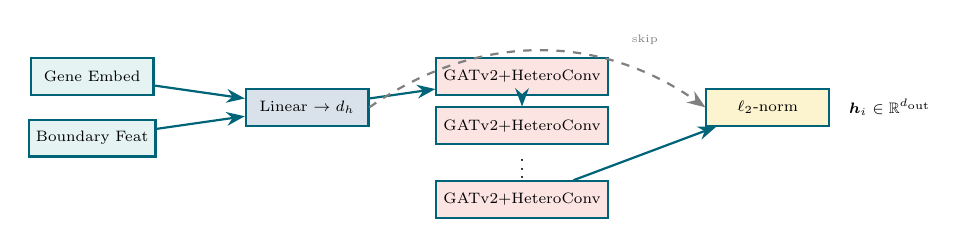
\begin{tikzpicture}[
  block/.style={rectangle, draw=tealdark, fill=tealaccent!10, thick, minimum width=2cm, minimum height=0.6cm, font=\scriptsize},
  arrow/.style={-{Stealth}, thick, tealdark},
  scale=0.78, every node/.style={scale=0.78}
]
  \node[block] (embed) at (0, 0) {Gene Embed};
  \node[block] (bd) at (0, -1) {Boundary Feat};
  \node[block, fill=deepblue!15] (lin) at (3.5, -0.5) {Linear $\to d_h$};
  \node[block, fill=coralaccent!15] (gat1) at (7, 0) {GATv2+HeteroConv};
  \node[block, fill=coralaccent!15] (gat2) at (7, -0.8) {GATv2+HeteroConv};
  \node[font=\small] at (7, -1.4) {$\vdots$};
  \node[block, fill=coralaccent!15] (gatN) at (7, -2) {GATv2+HeteroConv};
  \node[block, fill=goldaccent!20] (out) at (11, -0.5) {$\ell_2$-norm};
  \node[font=\scriptsize, right] at (12.2, -0.5) {$\vect{h}_i \in \Real^{d_{\text{out}}}$};

  \draw[arrow] (embed) -- (lin);
  \draw[arrow] (bd) -- (lin);
  \draw[arrow] (lin) -- (gat1);
  \draw[arrow] (gat1) -- (gat2);
  \draw[arrow] (gatN) -- (out);
  \draw[arrow, dashed, gray] (lin.east) to[bend left=35] (out.west);
  \node[font=\tiny, gray, above] at (9, 0.4) {skip};
\end{tikzpicture}
\end{center}

\vspace{0.1cm}

{\small\textbf{GATv2 attention} (per edge type $\phi$):}
\[
  \alpha_{ij}^{(\phi)} = \frac{\exp\big(\vect{a}^{\top}\text{LeakyReLU}(\mat{W}[\vect{h}_i \| \vect{h}_j])\big)}{\sum_{k \in \mathcal{N}_\phi(i)} \exp\big(\vect{a}^{\top}\text{LeakyReLU}(\mat{W}[\vect{h}_i \| \vect{h}_k])\big)}, \quad
  \vect{h}_i' = \sum_{\phi}\sum_{j} \alpha_{ij}^{(\phi)}\mat{W}_\phi \vect{h}_j
\]

\vspace{-0.1cm}
{\footnotesize $n_{\text{mid}} + 2$ layers, each with multi-head attention. Edge types: \texttt{tx-tx}, \texttt{tx-bd}, \texttt{bd-bd}.}
\end{frame}

\begin{frame}{v0.1.0 Loss: BCE Link Prediction (Baseline)}

\begin{block}{v0.1.0 --- Binary Cross-Entropy}
\vspace{-0.2cm}
\[
  \Lcal_{\text{BCE}} = -\!\sum_{(t_i, c_j)} \big[ y_{ij}\log\sigma(s_{ij}) + (1 - y_{ij})\log(1 - \sigma(s_{ij})) \big]
\]
\end{block}

\vspace{0.1cm}

{\small
\begin{itemize}\setlength\itemsep{2pt}
  \item $s_{ij} = \inner{f(t_i)}{f(c_j)}$ \quad (dot product of L2-normalized embeddings)
  \item Hard negatives from nearby cells (1:5 positive/negative ratio)
  \item Single global threshold $\theta$
\end{itemize}
}

\vspace{0.15cm}
\begin{alertblock}{Limitations Addressed in v0.2.0}
\begin{columns}[T]
\begin{column}{0.48\textwidth}
{\small
\begin{itemize}\setlength\itemsep{1pt}
  \item Single loss --- no embedding structure
  \item No biological priors (ME genes)
  \item Global threshold for all genes
\end{itemize}
}
\end{column}
\begin{column}{0.48\textwidth}
{\small
\begin{itemize}\setlength\itemsep{1pt}
  \item No recovery of unassigned transcripts
  \item Pandas/Dask data overhead
  \item \texttt{buffer()} only (no polygon shrink)
\end{itemize}
}
\end{column}
\end{columns}
\end{alertblock}
\end{frame}

% ============================================
% SECTION 2: MULTI-TASK LOSS
% ============================================
\section{Multi-Task Loss (NEW)}

\begin{frame}{Multi-Task Loss Overview \NEW}

\begin{block}{Combined Loss with Cosine-Scheduled Weights}
\vspace{-0.2cm}
\[
  \Lcal_{\text{main}} = w_{\text{tx}}(t)\,\Lcal_{\text{triplet}}^{\text{tx}} + w_{\text{bd}}(t)\,\Lcal_{\text{metric}}^{\text{bd}} + w_{\text{sg}}(t)\,\Lcal_{\text{triplet}}^{\text{sg}}
\]
\end{block}

\textbf{Weight scheduling} (cosine annealing per component):
\[
  \alpha(t) = \tfrac{1}{2}\big(1 + \cos(\pi t / T)\big), \qquad w_i(t) = w_i^{\text{end}} + (w_i^{\text{start}} - w_i^{\text{end}})\,\alpha(t)
\]

\begin{columns}[T]
\begin{column}{0.45\textwidth}
\begin{center}
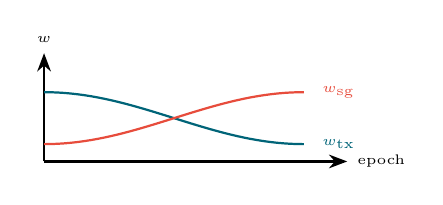
\begin{tikzpicture}[scale=0.55]
  \draw[-{Stealth}, thick] (0,0) -- (7,0) node[right] {\tiny epoch};
  \draw[-{Stealth}, thick] (0,0) -- (0,2.5) node[above] {\tiny $w$};
  \draw[thick, tealdark] plot[domain=0:6, samples=40] (\x, {0.4 + 1.2*0.5*(1+cos(deg(\x*3.14/6)))});
  \draw[thick, coralaccent] plot[domain=0:6, samples=40] (\x, {1.6 - 1.2*0.5*(1+cos(deg(\x*3.14/6)))});
  \node[tealdark, right, font=\tiny] at (6.2, 0.4) {$w_{\text{tx}}$};
  \node[coralaccent, right, font=\tiny] at (6.2, 1.6) {$w_{\text{sg}}$};
\end{tikzpicture}
\end{center}
\end{column}
\begin{column}{0.52\textwidth}
{\small
\begin{tabular}{@{}lll@{}}
\textbf{Term} & \textbf{Loss type} & \textbf{Margin} \\
\midrule
$\Lcal_{\text{tx}}$ & Transcript triplet & $m=0.3$ \\
$\Lcal_{\text{bd}}$ & Boundary metric & --- \\
$\Lcal_{\text{sg}}$ & Segmentation triplet & $m=0.4$ \\
\end{tabular}
}
\end{column}
\end{columns}
\end{frame}

\begin{frame}{Triplet Loss + FastTripletSelector \NEW}

\begin{block}{Triplet Margin Loss}
\vspace{-0.2cm}
\[
  \Lcal_{\text{triplet}} = \frac{1}{|\mathcal{A}|}\sum_{(a,p,n)} \max\!\big(0,\; \|\vect{h}_a - \vect{h}_p\|^2 - \|\vect{h}_a - \vect{h}_n\|^2 + m\big)
\]
\end{block}

\vspace{0.1cm}

\begin{columns}[T]
\begin{column}{0.48\textwidth}
\textbf{Cluster Similarity} $\mat{S} \in \Real^{K \times K}$:
{\small
\begin{enumerate}\setlength\itemsep{1pt}
  \item Phenograph/Louvain on boundary KNN
  \item $S_{ij}$ = Jaccard similarity of clusters
  \item Positive: $P(k) \propto S_{a_c, k}$
  \item Negative: $P(k) \propto -S_{a_c, k}$
\end{enumerate}
}
\end{column}
\begin{column}{0.48\textwidth}
\textbf{FastTripletSelector} --- $O(1)$ per sample:
{\small
\begin{enumerate}\setlength\itemsep{1pt}
  \item Build CDF: $\text{cdf}_k = \sum_{j \leq k} S_{a,j}/\sum S$
  \item Sample $u \sim \text{Unif}(0,1)$
  \item $k^* = \texttt{searchsorted}(\text{cdf}, u)$
  \item Pick random node from cluster $k^*$
\end{enumerate}
}

\vspace{0.1cm}
{\footnotesize Complexity: $O(N)$ total vs $O(NK)$ random rejection.}
\end{column}
\end{columns}
\end{frame}

\begin{frame}{Metric Loss: Boundary Embedding Quality \NEW}

\begin{block}{Metric Loss (MSE on Cosine Similarity)}
\vspace{-0.2cm}
\[
  \Lcal_{\text{metric}} = \mathbb{E}\!\big[\text{MSE}(\cos(\vect{h}_a, \vect{h}_p),\; 1 - d_{ap}) + \text{MSE}(\cos(\vect{h}_a, \vect{h}_n),\; 1 - d_{an})\big]
\]
\end{block}

where $d_{ap} = 1 - S_{c_a, c_p}$ is cluster dissimilarity from phenograph.

\vspace{0.2cm}

\begin{columns}[T]
\begin{column}{0.48\textwidth}
\textbf{Intuition:}
{\small
\begin{itemize}\setlength\itemsep{1pt}
  \item Similar cell embeddings $\to$ high cosine similarity
  \item Dissimilar cells $\to$ low cosine similarity
  \item Phenograph clustering = soft labels
\end{itemize}
}
\end{column}
\begin{column}{0.48\textwidth}
\textbf{Phenograph pipeline:}
{\small
\begin{enumerate}\setlength\itemsep{1pt}
  \item Cell $\times$ gene count matrix
  \item PCA $\to \Real^{d}$
  \item KNN graph ($k=30$)
  \item Louvain ($\rho = 2$--$3$)
  \item $\mat{S}$: Jaccard between communities
\end{enumerate}
}
\end{column}
\end{columns}
\end{frame}

\begin{frame}{Alignment Loss: ME Gene Constraints \NEW}

\begin{block}{Contrastive Loss on tx--tx Edges}
\vspace{-0.2cm}
\[
  \Lcal_{\text{align}} = \underbrace{\sum_{(i,j) \in \mathcal{P}} (1 - s_{ij})^2}_{\text{same-gene: attract}} + \underbrace{\sum_{(i,j) \in \mathcal{N}} \max(s_{ij} - m,\; 0)^2}_{\text{ME-gene: repel}}
\]
\end{block}

{\small
$s_{ij} = \cos(\vect{h}_i, \vect{h}_j)$, \quad $m = 0.2$, \quad $|\mathcal{P}| \leq 3|\mathcal{N}|$ (subsample positives)
}

\vspace{0.15cm}

\begin{columns}[T]
\begin{column}{0.48\textwidth}
\textbf{ME Gene Discovery:}
{\small
\begin{enumerate}\setlength\itemsep{1pt}
  \item Rank genes by expression per cell type
  \item Select top 10\% expressed in $\geq$30\% cells
  \item Filter: $\text{expr}_{\text{in}} > 0.25$, $\text{expr}_{\text{out}} < 0.03$
  \item Cross-type pairs $\to$ ME set
\end{enumerate}
}
\end{column}
\begin{column}{0.48\textwidth}
\textbf{Validation --- MECR:}
\[
  \text{MECR}(g_1, g_2) = \frac{P(g_1 \wedge g_2)}{P(g_1 \vee g_2)}
\]
{\small Lower $=$ better. $< 0.15$ is good.

Alignment loss $\Rightarrow$ MECR $\downarrow$ 10--30\%.}
\end{column}
\end{columns}

\vspace{0.15cm}
\begin{exampleblock}{CLI Usage}
\centering
{\small\texttt{segger segment -i data/ -o out/ --alignment-loss --scrna-reference-path ref.h5ad}}
\end{exampleblock}
\end{frame}

\begin{frame}[fragile]{Vectorized ME Gene Matching \PERF}

\textbf{Problem:} Given $|\edges|$ tx--tx edges and $|\text{ME}|$ gene pairs, find ME edges efficiently.

\vspace{0.15cm}

\begin{columns}[T]
\begin{column}{0.48\textwidth}
\textbf{v0.1.0:} $O(|\edges| \cdot |\text{ME}|)$
\begin{lstlisting}[language=Python]
for i, (src, dst) in enumerate(edges):
    for g1, g2 in me_pairs:  # SLOW
        if genes[src]==g1 and genes[dst]==g2:
            is_me[i] = True
\end{lstlisting}
\end{column}

\begin{column}{0.48\textwidth}
\textbf{v0.2.0:} $O(|\edges| + |\text{ME}|)$
\begin{lstlisting}[language=Python]
# Cantor pairing function
me_keys = me_min * G + me_max
edge_min = torch.minimum(src_g, dst_g)
edge_max = torch.maximum(src_g, dst_g)
edge_keys = edge_min * G + edge_max
is_me = torch.isin(edge_keys, me_keys)
\end{lstlisting}
\end{column}
\end{columns}

\vspace{0.15cm}

{\small
\textbf{Key:} Map unordered pair $(g_a, g_b)$ to scalar: $\text{key} = \min(g_a, g_b) \cdot G_{\max} + \max(g_a, g_b)$

Then \texttt{torch.isin()} for $O(1)$ amortized lookup. \alert{10--50$\times$ speedup.}
}
\end{frame}

\begin{frame}{Loss Combination Modes \NEW}

\begin{columns}[T]
\begin{column}{0.48\textwidth}
\begin{block}{Interpolate (Default)}
\vspace{-0.2cm}
\[
  \Lcal = (1 - w_a)\Lcal_{\text{main}} + w_a\Lcal_{\text{align}}
\]
{\small
\begin{itemize}\setlength\itemsep{1pt}
  \item Total scale $\approx$ constant
  \item Main loss fades as alignment ramps
  \item Recommended for most cases
\end{itemize}
}
\end{block}
\end{column}
\begin{column}{0.48\textwidth}
\begin{alertblock}{Additive}
\vspace{-0.2cm}
\[
  \Lcal = \Lcal_{\text{main}} + w_a\Lcal_{\text{align}}
\]
{\small
\begin{itemize}\setlength\itemsep{1pt}
  \item Total scale increases over training
  \item May need LR adjustment
  \item For aggressive ME enforcement
\end{itemize}
}
\end{alertblock}
\end{column}
\end{columns}

\vspace{0.15cm}

\textbf{Full v0.2.0 loss:}
\[
  \Lcal_{\text{v2}} = \underbrace{w_t\Lcal_{\text{tri}}^{t}}_{\text{tx}} + \underbrace{w_b\Lcal_{\text{met}}^{b}}_{\text{bd}} + \underbrace{w_s\Lcal_{\text{tri}}^{s}}_{\text{seg}} + \underbrace{w_a\Lcal_{\text{align}}}_{\text{ME}}
\]

\vspace{0.1cm}
\begin{exampleblock}{CLI}
\centering
{\small\texttt{segger segment -i data/ -o out/ --loss-combination-mode interpolate}}
\end{exampleblock}
\end{frame}

% ============================================
% SECTION 3: FRAGMENT MODE
% ============================================
\section{Fragment Mode (NEW)}

\begin{frame}{Fragment Mode: Recovering Unassigned Transcripts \NEW}

\textbf{Problem:} Transcripts with $\max_j s_{ij} < \theta$ remain unassigned after segmentation.

\vspace{0.15cm}

\begin{block}{Algorithm}
{\small
\begin{enumerate}\setlength\itemsep{1pt}
  \item \textbf{Identify} unassigned: $\Tcal_u = \{t_i : \text{seg\_cell\_id}(t_i) = \varnothing\}$
  \item \textbf{Filter} tx--tx edges: $\edges_u = \{(t_i, t_j) \in \edges_{TT} : t_i, t_j \in \Tcal_u\}$
  \item \textbf{Threshold:} $\edges_u' = \{(i,j) \in \edges_u : s_{ij} \geq \theta_f\}$
  \item \textbf{Connected components:} $\{C_1, \ldots\} = \text{CC}(\Tcal_u, \edges_u')$
  \item \textbf{Size filter:} keep $C_k$ if $|C_k| \geq n_{\min}$ (default: 5)
  \item \textbf{Assign:} $\text{seg\_cell\_id}(t_i) = \texttt{"frag-}k\texttt{"}$ for $t_i \in C_k$
\end{enumerate}
}
\end{block}

\vspace{0.1cm}

\begin{columns}[T]
\begin{column}{0.48\textwidth}
{\small
\textbf{Auto-threshold:} Li + Yen histogram methods on similarity distribution. Fallback: median.
}
\end{column}
\begin{column}{0.48\textwidth}
\begin{exampleblock}{CLI}
{\small\texttt{segger segment -i data/ -o out/ \textbackslash\\
\quad --fragment-mode \textbackslash\\
\quad --fragment-min-transcripts 10}}
\end{exampleblock}
\end{column}
\end{columns}
\end{frame}

\begin{frame}[fragile]{GPU-Accelerated Connected Components \NEW}

\begin{columns}[T]
\begin{column}{0.48\textwidth}
\begin{block}{GPU Path (RAPIDS/CuPy)}
\begin{lstlisting}[language=Python]
ids = cp.unique(cp.concat([src, dst]))
src_i = cp.searchsorted(ids, src)
dst_i = cp.searchsorted(ids, dst)

# Symmetric CSR
rows = cp.concat([src_i, dst_i])
cols = cp.concat([dst_i, src_i])
A = cp_csr((ones, (rows, cols)), (n, n))

# GPU connected components
n_cc, labels = cc_gpu(A, directed=False)
valid = cp.bincount(labels) >= n_min
\end{lstlisting}
\end{block}
\end{column}

\begin{column}{0.48\textwidth}
\begin{block}{CPU Fallback (SciPy)}
\begin{lstlisting}[language=Python]
id_map = {v: i for i, v
          in enumerate(unique_ids)}
src_i = [id_map[s] for s in src]
dst_i = [id_map[d] for d in dst]

A = csr_matrix((data, (rows, cols)),
               shape=(n, n))
n_cc, labels = cc_cpu(A, directed=False)
\end{lstlisting}
\end{block}

\vspace{0.1cm}
{\small\textbf{Complexity:} $O(|\Tcal_u| + |\edges_u'|)$ \\
GPU: $\sim O(|\Tcal_u|/P)$ with $P$ cores}
\end{column}
\end{columns}

\vspace{0.1cm}
{\footnotesize\textbf{Post-hoc similarity:} Chunked cosine similarity from gene embeddings (256\,MB chunks).}
\end{frame}

% ============================================
% SECTION 4: ADAPTIVE THRESHOLDING
% ============================================
\section{Adaptive Thresholding (NEW)}

\begin{frame}{Per-Gene Adaptive Thresholding \NEW}

\begin{columns}[T]
\begin{column}{0.48\textwidth}
\begin{block}{Fixed Threshold (v0.1.0)}
\vspace{-0.2cm}
\[
  \hat{c}(t_i) = \begin{cases} \argmax_j s_{ij} & \max_j s_{ij} \geq \theta \\ \varnothing & \text{otherwise} \end{cases}
\]
Single $\theta$ for all genes.
\end{block}

\begin{alertblock}{Per-Gene Auto (v0.2.0)}
For each gene $g$:
\vspace{-0.2cm}
\[
  \theta_g = \min(\theta_g^{\text{Li}},\, \theta_g^{\text{Yen}})
\]
Fallback: $\theta_g = \text{median}(s_g)$.
\end{alertblock}
\end{column}

\begin{column}{0.48\textwidth}
{\small
\textbf{Li:} Minimize cross-entropy
\[
  \theta^{\text{Li}} = \argmin_\theta \sum_x p(x) \log\frac{p(x)}{q_\theta(x)}
\]

\textbf{Yen:} Maximum correlation
\[
  \theta^{\text{Yen}} = \argmax_\theta \frac{(\sum_{x \leq \theta} x p(x))^2}{\sum_{x \leq \theta} p(x)}
\]

\textbf{Memory:} $|S_g| > 10^7 \Rightarrow$ subsample.

Both methods robust to multi-modal distributions.
}
\end{column}
\end{columns}

\vspace{0.1cm}
\begin{exampleblock}{CLI --- Fixed vs Auto}
\centering
{\small\texttt{segger segment -i data/ -o out/ --min-similarity 0.5}\ \ \textit{(fixed)} \\
\texttt{segger segment -i data/ -o out/}\ \ \textit{(auto per-gene, default)}}
\end{exampleblock}
\end{frame}

% ============================================
% SECTION 5: DELAUNAY BOUNDARIES
% ============================================
\section{Delaunay Boundaries (NEW)}

\begin{frame}{Two-Phase Delaunay Boundary Extraction \NEW}

Construct cell boundaries \alert{de novo} from transcript point clouds.

\vspace{0.1cm}

\begin{columns}[T]
\begin{column}{0.52\textwidth}
{\small
\textbf{Phase 1: Long Edge Removal}
\begin{enumerate}\setlength\itemsep{1pt}
  \item $d_{\max}$ = max nearest-neighbor distance
  \item Find boundary edges ($<2$ incident simplices)
  \item Remove if $\ell > 2\,d_{\max}$
  \item Propagate: deleted simplices $\to$ new boundary
\end{enumerate}

\textbf{Phase 2: Extreme Angle Removal}
\[
  \text{Remove if } \begin{cases}
    \ell > 1.5d_{\max} \wedge \alpha > 90^{\circ} \\
    \text{or } \alpha > 168.75^{\circ}
  \end{cases}
\]
}
\end{column}

\begin{column}{0.42\textwidth}
\begin{center}
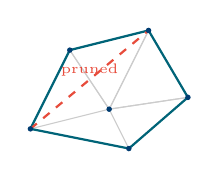
\begin{tikzpicture}[scale=0.5]
  \coordinate (A) at (0,0);
  \coordinate (B) at (2,0.5);
  \coordinate (C) at (1,2);
  \coordinate (D) at (3,2.5);
  \coordinate (E) at (4,0.8);
  \coordinate (F) at (2.5,-0.5);
  \draw[gray!40] (A)--(B)--(C)--cycle;
  \draw[gray!40] (B)--(C)--(D)--cycle;
  \draw[gray!40] (B)--(D)--(E)--cycle;
  \draw[gray!40] (B)--(E)--(F)--cycle;
  \draw[thick, tealdark] (A)--(C)--(D)--(E)--(F)--(A);
  \draw[thick, coralaccent, dashed] (A)--(D);
  \node[coralaccent, font=\tiny] at (1.5, 1.5) {pruned};
  \foreach \p in {A,B,C,D,E,F} \fill[deepblue] (\p) circle (0.07);
\end{tikzpicture}
\end{center}

{\small
\textbf{Cycle detection:} DFS on boundary graph $\to$ Shapely polygons.

\textbf{Complexity:} $O(n \log n)$ (Delaunay dominates).

\textbf{Angles:} Vectorized --- all triangles at once.
}
\end{column}
\end{columns}
\end{frame}

% ============================================
% SECTION 6: ENGINEERING CHANGES
% ============================================
\section{Engineering Changes}

\begin{frame}[fragile]{Polars Replacing Pandas/Dask \CHANGED}

\begin{columns}[T]
\begin{column}{0.48\textwidth}
{\small
\textbf{Why Polars:}
\begin{itemize}\setlength\itemsep{1pt}
  \item Lazy evaluation + query optimization
  \item Streaming mode for $>$10M rows
  \item 2--3$\times$ less memory than Pandas
  \item Apache Arrow columnar backend
  \item Rust-based parallelism
\end{itemize}
}

\begin{lstlisting}[language=Python]
# Auto-streaming for large files
lf = pl.scan_parquet("transcripts.pq")
result = lf.filter(
    pl.col("qv") >= 20
).group_by("cell_id").agg(
    pl.count()
).collect(streaming=True)
\end{lstlisting}
\end{column}

\begin{column}{0.48\textwidth}
\textbf{cuSpatial Replacing cuML:}
{\small
\begin{itemize}\setlength\itemsep{1pt}
  \item GPU-native point-in-polygon
  \item Quadtree spatial indexing
  \item Polygon area/centroid ops
\end{itemize}
}

\vspace{0.15cm}
\begin{exampleblock}{GPU/CPU Fallback}
{\scriptsize
\begin{tabular}{@{}l@{$\;\to\;$}l@{}}
cuSpatial & GeoPandas \\
CuPy sparse & SciPy sparse \\
cuML & scanpy/sklearn \\
\end{tabular}

All GPU ops auto-fallback to CPU.
}
\end{exampleblock}
\end{column}
\end{columns}
\end{frame}

\begin{frame}[fragile]{Vectorized Batch Normalization \PERF}

\textbf{Positional encoding:} Sinusoidal 2D spatial embeddings:
\[
  \text{PE}(p, 2k) = \sin\!\big(p / 10000^{2k/d}\big), \quad
  \text{PE}(p, 2k{+}1) = \cos\!\big(p / 10000^{2k/d}\big)
\]

\vspace{0.1cm}

\begin{columns}[T]
\begin{column}{0.48\textwidth}
\textbf{v0.1.0} --- per-sample loop, $O(B \cdot N \cdot d)$:
\begin{lstlisting}[language=Python]
for b in range(num_batches):  # SLOW
    mask = (batch == b)
    pos[mask] = (pos[mask] - pos[mask].min(0)
                ) / (pos[mask].max(0)
                     - pos[mask].min(0))
\end{lstlisting}
\end{column}
\begin{column}{0.48\textwidth}
\textbf{v0.2.0} --- scatter ops, $O(N \cdot d)$:
\begin{lstlisting}[language=Python]
mins, _ = scatter_min(pos, batch,
                      dim=0, dim_size=B)
maxs, _ = scatter_max(pos, batch,
                      dim=0, dim_size=B)
pos_norm = (pos - mins[batch]) / (
    maxs[batch] - mins[batch]
).clamp_min(1e-8)
\end{lstlisting}
\end{column}
\end{columns}

\vspace{0.1cm}
{\small\alert{10--100$\times$ speedup}. Eliminates per-batch Python loop entirely.}
\end{frame}

\begin{frame}{Polygon Scaling: \texttt{scale()} vs \texttt{buffer()} \CHANGED}

\begin{columns}[T]
\begin{column}{0.48\textwidth}
\begin{center}
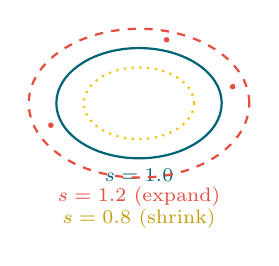
\begin{tikzpicture}[scale=0.7]
  \draw[thick, tealdark] (0,0) ellipse (1.5 and 1.0);
  \node[tealdark, font=\scriptsize] at (0, -1.3) {$s = 1.0$};
  \draw[thick, coralaccent, dashed] (0,0) ellipse (2.0 and 1.35);
  \node[coralaccent, font=\scriptsize] at (0, -1.7) {$s = 1.2$ (expand)};
  \draw[thick, goldaccent, dotted] (0,0) ellipse (1.0 and 0.65);
  \node[goldaccent!80!black, font=\scriptsize] at (0, -2.1) {$s = 0.8$ (shrink)};
  \fill[coralaccent] (1.7, 0.3) circle (0.05);
  \fill[coralaccent] (-1.6, -0.4) circle (0.05);
  \fill[coralaccent] (0.5, 1.15) circle (0.05);
\end{tikzpicture}
\end{center}
\end{column}

\begin{column}{0.48\textwidth}
{\small
\textbf{v0.1.0:} \texttt{buffer()} --- isotropic dilation only

\textbf{v0.2.0:} \texttt{scale()} --- expand \textbf{and} shrink
}

\[
  B_j^{(s)} = \text{scale}(B_j, s), \quad s \in (0, \infty)
\]

{\small
\textbf{Recommended settings:}
\begin{itemize}\setlength\itemsep{1pt}
  \item Training: $s = 1.0$
  \item Prediction: $s = 1.0$--$1.5$
  \item High-precision: $s < 1.0$
\end{itemize}
}
\end{column}
\end{columns}

\vspace{0.15cm}
\begin{exampleblock}{CLI}
\centering
{\small\texttt{segger segment -i data/ -o out/ --prediction-scale-factor 1.2}}
\end{exampleblock}
\end{frame}

% ============================================
% SECTION 7: CHECKPOINT & I/O
% ============================================
\section{Checkpoint \& I/O (NEW)}

\begin{frame}[fragile]{Simplified Checkpoint Workflows \NEW}

\begin{center}
{\small
\renewcommand{\arraystretch}{1.2}
\begin{tabular}{@{}>{\bfseries\ttfamily}l p{3.5cm} p{5cm}@{}}
\toprule
\textrm{\textbf{Mode}} & \textbf{Description} & \textbf{Vocabulary Handling} \\
\midrule
train & Fresh training & Embeddings from data vocab \\
finetune & Load weights, reset optim & Auto-remap: shared $\to$ keep, new $\to$ Xavier \\
predict & Skip training & Auto-filter data to checkpoint genes \\
\bottomrule
\end{tabular}
}
\end{center}

\vspace{0.15cm}

\begin{columns}[T]
\begin{column}{0.48\textwidth}
{\small
\textbf{Vocab remapping} (finetune):
\vspace{-0.15cm}
\begin{align*}
  V_{\text{shared}} &= V_{\text{ckpt}} \cap V_{\text{data}} \\
  V_{\text{new}} &= V_{\text{data}} \setminus V_{\text{ckpt}}
\end{align*}
Gene embeddings exported to \texttt{gene\_embeddings.parquet} by default.
}
\end{column}
\begin{column}{0.48\textwidth}
\begin{exampleblock}{CLI Examples}
\begin{lstlisting}[language=bash]
# Predict from checkpoint
segger segment -i data/ -o out/ \
  --checkpoint-path model.ckpt \
  --checkpoint-mode predict

# Finetune on new dataset
segger segment -i data/ -o out/ \
  --checkpoint-path model.ckpt \
  --checkpoint-mode finetune
\end{lstlisting}
\end{exampleblock}
\end{column}
\end{columns}

\vspace{0.05cm}
{\footnotesize\textit{Removed:} \texttt{--vocab-mode}, \texttt{--checkpoint-vocab}, \texttt{--filter-to-checkpoint-vocab} (all auto).}
\end{frame}

\begin{frame}[fragile]{I/O: SpatialData, AnnData, Quality Filters \NEW}

\begin{columns}[T]
\begin{column}{0.48\textwidth}
\textbf{Output formats:}
{\small
\begin{itemize}\setlength\itemsep{1pt}
  \item \texttt{segger\_raw}: Parquet predictions
  \item \texttt{merged}: Transcripts + assignments
  \item \texttt{spatialdata}: SpatialData Zarr (SOPA-compatible)
  \item \texttt{anndata}: Cell $\times$ gene \texttt{.h5ad}
  \item \texttt{all}: Everything
\end{itemize}
}

\vspace{0.1cm}
\textbf{Platform quality filters:}

{\scriptsize
\begin{tabular}{@{}lll@{}}
\textbf{Platform} & \textbf{Field} & \textbf{Default} \\
\midrule
Xenium & \texttt{qv} & $\geq 20$ \\
CosMx & Controls & Remove \\
MERSCOPE & Blanks & Remove \\
\end{tabular}
}
\end{column}

\begin{column}{0.48\textwidth}
\begin{exampleblock}{CLI Examples}
\begin{lstlisting}[language=bash]
# Output as SpatialData Zarr
segger segment -i data/ -o out/ \
  --output-format spatialdata

# Export to Xenium Explorer
segger export \
  -s predictions.parquet \
  -i /path/to/xenium/ \
  -o /export/ --num-workers 4

# Input from SpatialData
segger segment \
  -i data.zarr \
  --input-format spatialdata \
  -o out/
\end{lstlisting}
\end{exampleblock}
\end{column}
\end{columns}
\end{frame}

% ============================================
% SECTION 8: PERFORMANCE
% ============================================
\section{Performance}

\begin{frame}{Vectorization \& Scalability Summary}

\begin{center}
{\small
\renewcommand{\arraystretch}{1.15}
\begin{tabular}{@{}l l l c@{}}
\toprule
\textbf{Operation} & \textbf{v0.1.0} & \textbf{v0.2.0} & \textbf{Speedup} \\
\midrule
Batch norm & Per-sample loop & \texttt{scatter\_min/max} & \alert{10--100$\times$} \\
ME matching & Per-edge loop & Cantor hash + \texttt{isin} & \alert{10--50$\times$} \\
Triplet sampling & Random rejection & FastTripletSelector & \alert{$\sim$5$\times$} \\
Data loading & Pandas + Dask & Polars LazyFrames & \alert{2--3$\times$} \\
\bottomrule
\end{tabular}
}
\end{center}

\vspace{0.2cm}

\begin{columns}[T]
\begin{column}{0.48\textwidth}
\textbf{Training features:}
{\small
\begin{itemize}\setlength\itemsep{1pt}
  \item Mixed precision: \texttt{16-mixed}, \texttt{bf16-mixed}
  \item LR schedulers: cosine, OneCycle
  \item Early stopping
  \item Tile-based: 50K--100K tx/tile
\end{itemize}
}
\end{column}
\begin{column}{0.48\textwidth}
\textbf{GPU/CPU dual path:}
{\small
\begin{itemize}\setlength\itemsep{1pt}
  \item CuPy $\to$ SciPy (fragment CC)
  \item cuSpatial $\to$ GeoPandas (geometry)
  \item cuML $\to$ scanpy (clustering)
  \item Auto 3D detection
\end{itemize}
}
\end{column}
\end{columns}

\vspace{0.15cm}
\begin{exampleblock}{CLI --- Training Options}
\centering
{\small\texttt{segger segment -i data/ -o out/ --precision 16-mixed --lr-scheduler cosine}}
\end{exampleblock}
\end{frame}

% ============================================
% SECTION 9: HPO
% ============================================
\section{HPO (NEW)}

\begin{frame}[fragile]{Optuna-Based Hyperparameter Optimization \NEW}

\begin{columns}[T]
\begin{column}{0.48\textwidth}
{\small
\textbf{Features:}
\begin{itemize}\setlength\itemsep{1pt}
  \item Multi-objective: up to 5 objectives
  \item Samplers: TPE, NSGA-III, CMA-ES, Random
  \item Pruner: Hyperband (3$\times$ faster)
  \item SQLite persistence (resume-able)
  \item Multi-fidelity (10--20\% data first)
\end{itemize}

\textbf{Search space:}
\begin{itemize}\setlength\itemsep{1pt}
  \item Architecture: channels, layers, heads
  \item Training: LR, scheduler, loss
  \item Graph: $k$, dist, scale factor
  \item Loss: weights, margins
\end{itemize}
}
\end{column}

\begin{column}{0.48\textwidth}
\begin{exampleblock}{CLI Examples}
\begin{lstlisting}[language=bash]
# Basic HPO (50 trials)
segger hpo -i data/ -o results/ \
  --n-trials 50

# Multi-objective with NSGA-III
segger hpo -i data/ -o results/ \
  --n-objectives 5 --sampler nsga3

# Persistent study (resume-able)
segger hpo -i data/ -o results/ \
  --storage sqlite:///hpo.db

# Smart two-stage workflow
segger hpo -i data/ -o results/ \
  --workflow smart --n-trials 50
  # Stage 1: 50 trials on 20% data
  # Stage 2: top 10 on full data

# View results
optuna-dashboard sqlite:///hpo.db
\end{lstlisting}
\end{exampleblock}
\end{column}
\end{columns}
\end{frame}

% ============================================
% SECTION 10: COMPARISON
% ============================================
\section{Summary}

\begin{frame}{v0.1.0 vs v0.2.0: Complete Comparison}

\begin{center}
\renewcommand{\arraystretch}{1.1}
{\scriptsize
\begin{tabular}{@{}l l l@{}}
\toprule
\textbf{Feature} & \textbf{v0.1.0} & \textbf{v0.2.0} \\
\midrule
\rowcolor{lightgray} Data processing & Pandas + Dask & \textbf{Polars} (2--3$\times$ faster) \\
GPU geometry & RAPIDS cuML & \textbf{cuSpatial} (native PiP) \\
\rowcolor{lightgray} Loss function & BCE only & \textbf{BCE + Triplet + Metric + Alignment} \\
Triplet sampling & Random & \textbf{FastTripletSelector} (inverse CDF) \\
\rowcolor{lightgray} Biological priors & None & \textbf{ME gene alignment loss} \\
Gene embeddings & One-hot / external & \textbf{Learned + PCA + exported} \\
\rowcolor{lightgray} Batch normalization & Per-sample loop & \textbf{scatter\_min/max} (10--100$\times$) \\
Polygon scaling & \texttt{buffer()} only & \textbf{\texttt{scale()}} (expand + shrink) \\
\rowcolor{lightgray} Similarity threshold & Global $\theta$ & \textbf{Per-gene Li + Yen auto} \\
Unassigned transcripts & Discarded & \textbf{Fragment mode} (GPU CC) \\
\rowcolor{lightgray} Boundary construction & External only & \textbf{Delaunay} (de novo) \\
Checkpoint system & Manual vocab & \textbf{Auto} (train/finetune/predict) \\
\rowcolor{lightgray} Weight scheduling & Fixed & \textbf{Cosine annealing} \\
Export formats & Parquet & \textbf{Zarr, SpatialData, AnnData, Explorer} \\
\rowcolor{lightgray} Quality filtering & Manual & \textbf{Platform-specific} (Xenium/CosMx/MERSCOPE) \\
HPO & None & \textbf{Optuna} (multi-objective, multi-fidelity) \\
\rowcolor{lightgray} Training precision & FP32 only & \textbf{FP16/BF16 mixed precision} \\
\bottomrule
\end{tabular}
}
\end{center}
\end{frame}

\begin{frame}{v0.2.0 Pipeline Overview}

\begin{center}
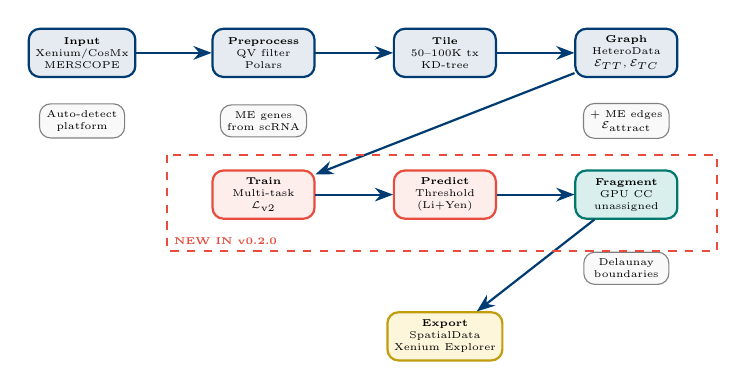
\begin{tikzpicture}[
  stage/.style={rectangle, draw=deepblue, fill=deepblue!10, thick, rounded corners, minimum width=1.8cm, minimum height=0.85cm, font=\tiny, align=center},
  substage/.style={rectangle, draw=gray, fill=gray!5, rounded corners, font=\tiny, align=center, minimum width=1.5cm},
  arrow/.style={-{Stealth}, thick, deepblue},
  scale=0.72, every node/.style={scale=0.72}
]
  \node[stage] (input) at (0, 0) {\textbf{Input}\\Xenium/CosMx\\MERSCOPE};
  \node[stage] (preproc) at (3.2, 0) {\textbf{Preprocess}\\QV filter\\Polars};
  \node[stage] (tile) at (6.4, 0) {\textbf{Tile}\\50--100K tx\\KD-tree};
  \node[stage] (graph) at (9.6, 0) {\textbf{Graph}\\HeteroData\\$\edges_{TT}, \edges_{TC}$};

  \node[stage, fill=coralaccent!10, draw=coralaccent] (train) at (3.2, -2.5) {\textbf{Train}\\Multi-task\\$\Lcal_{\text{v2}}$};
  \node[stage, fill=coralaccent!10, draw=coralaccent] (pred) at (6.4, -2.5) {\textbf{Predict}\\Threshold\\(Li+Yen)};
  \node[stage, fill=tealaccent!15, draw=tealaccent!80!black] (frag) at (9.6, -2.5) {\textbf{Fragment}\\GPU CC\\unassigned};

  \node[stage, fill=goldaccent!15, draw=goldaccent!80!black] (export) at (6.4, -5) {\textbf{Export}\\SpatialData\\Xenium Explorer};

  \draw[arrow] (input) -- (preproc);
  \draw[arrow] (preproc) -- (tile);
  \draw[arrow] (tile) -- (graph);
  \draw[arrow] (graph) -- (train);
  \draw[arrow] (train) -- (pred);
  \draw[arrow] (pred) -- (frag);
  \draw[arrow] (frag) -- (export);

  \node[substage] at (0, -1.2) {Auto-detect\\platform};
  \node[substage] at (3.2, -1.2) {ME genes\\from scRNA};
  \node[substage] at (9.6, -1.2) {+ ME edges\\$\edges_{\text{attract}}$};
  \node[substage] at (9.6, -3.8) {Delaunay\\boundaries};

  \draw[thick, coralaccent, dashed] (1.5, -1.8) rectangle (11.2, -3.5);
  \node[coralaccent, font=\tiny\bfseries, above right] at (1.5, -3.5) {NEW IN v0.2.0};
\end{tikzpicture}
\end{center}
\end{frame}

\begin{frame}{Key Equations Summary}

{\small
\begin{align}
  \text{\textbf{Assignment:}} \quad & \hat{c}(t_i) = \argmax_j \inner{f(t_i)}{f(c_j)} \;\text{s.t.}\; s_{ij} \geq \theta_g \tag{1} \\[4pt]
  \text{\textbf{BCE (v0.1):}} \quad & \Lcal_{\text{BCE}} = -\!\sum \big[y\log\sigma(s) + (1{-}y)\log(1{-}\sigma(s))\big] \tag{2} \\[4pt]
  \text{\textbf{Triplet:}} \quad & \Lcal_{\text{tri}} = \frac{1}{|\mathcal{A}|}\!\sum\max\!\big(0, \|h_a{-}h_p\|^2 - \|h_a{-}h_n\|^2 + m\big) \tag{3} \\[4pt]
  \text{\textbf{Metric:}} \quad & \Lcal_{\text{met}} = \mathbb{E}\big[\text{MSE}(\cos(h_a,h_p), 1{-}d) + \text{MSE}(\cos(h_a,h_n), 1{-}d)\big] \tag{4} \\[4pt]
  \text{\textbf{Alignment:}} \quad & \Lcal_{\text{align}} = \!\sum_{\mathcal{P}}(1{-}s)^2 + \!\sum_{\mathcal{N}}\max(s{-}m, 0)^2 \tag{5} \\[4pt]
  \text{\textbf{v0.2.0:}} \quad & \Lcal = (1{-}w_a)\big[w_t\Lcal_{\text{tri}}^t + w_b\Lcal_{\text{met}}^b + w_s\Lcal_{\text{tri}}^s\big] + w_a\Lcal_{\text{align}} \tag{6} \\[4pt]
  \text{\textbf{Schedule:}} \quad & w_i(t) = w_i^{\text{end}} + (w_i^{\text{start}} - w_i^{\text{end}}) \cdot \tfrac{1}{2}(1 + \cos(\pi t / T)) \tag{7}
\end{align}
}
\end{frame}

% ============================================
% THANK YOU
% ============================================

\begin{frame}[plain,fragile]
  \begin{center}
    \vspace{1cm}
    {\Huge \textbf{Segger v0.2.0}}

    \vspace{0.5cm}

    {\Large Install \& Get Started}

    \vspace{0.5cm}

    \begin{columns}
      \begin{column}{0.45\textwidth}
        \centering
        {\small\textbf{Install:}}\\[0.1cm]
        \texttt{pip install segger}\\[0.3cm]
        {\small\textbf{Basic segmentation:}}\\[0.1cm]
        {\small\texttt{segger segment -i data/ -o out/}}\\[0.3cm]
        {\small\textbf{With ME gene alignment:}}\\[0.1cm]
        {\scriptsize\texttt{segger segment -i data/ -o out/ \textbackslash}}\\
        {\scriptsize\texttt{\ \ --alignment-loss \textbackslash}}\\
        {\scriptsize\texttt{\ \ --scrna-reference-path ref.h5ad}}
      \end{column}

      \begin{column}{0.45\textwidth}
        \centering
        {\small\textbf{Export to Xenium Explorer:}}\\[0.1cm]
        {\small\texttt{segger export -s seg.pq -o exp/}}\\[0.3cm]
        {\small\textbf{From checkpoint:}}\\[0.1cm]
        {\scriptsize\texttt{segger segment -i data/ -o out/ \textbackslash}}\\
        {\scriptsize\texttt{\ \ --checkpoint-path model.ckpt \textbackslash}}\\
        {\scriptsize\texttt{\ \ --checkpoint-mode predict}}\\[0.3cm]
        {\small\textbf{HPO:}}\\[0.1cm]
        {\small\texttt{segger hpo -i data/ -o hpo/}}
      \end{column}
    \end{columns}

    \vspace{0.6cm}

    {\footnotesize Segger: scalable graph neural network cell segmentation (2025)}
  \end{center}
\end{frame}

% ============================================
% BACKUP SLIDES
% ============================================
\appendix

\begin{frame}{Backup: Hyperparameter Recommendations}

\begin{center}
\renewcommand{\arraystretch}{1.2}
{\small
\begin{tabular}{@{}l l l@{}}
\toprule
\textbf{Parameter} & \textbf{Heuristic} & \textbf{Range} \\
\midrule
\texttt{transcripts\_max\_k} & 90th pctl of local density & 5--15 \\
\texttt{transcripts\_max\_dist} & $\approx 0.5\times$ median nuclear radius & 5--10\,$\mu$m \\
\texttt{prediction\_scale\_factor} & Expand for edge tx & 1.0--1.5 \\
\texttt{tile\_size} & 50K--100K transcripts & By VRAM \\
\texttt{hidden\_channels} & Model capacity & 32--128 \\
\texttt{n\_heads} & Attention diversity & 3--8 \\
\texttt{alignment\_loss\_weight\_end} & ME strength & 0.05--0.2 \\
\texttt{fragment\_min\_transcripts} & Min component size & 5--20 \\
\texttt{learning\_rate} & With scheduler & $10^{-4}$--$10^{-3}$ \\
\bottomrule
\end{tabular}
}
\end{center}
\end{frame}

\begin{frame}[fragile]{Backup: FastTripletSelector Algorithm}

\begin{block}{FastTripletSelector}
{\footnotesize
\textbf{Input:} Embeddings $\mat{H}$, cluster labels $\vect{c}$, similarity $\mat{S} \in \Real^{K \times K}$ \\
\textbf{Output:} Triplets $(a, p, n)$ for each anchor
}
\end{block}

\vspace{-0.1cm}
\begin{lstlisting}[language=Python, basicstyle=\ttfamily\tiny]
# 1. Build per-cluster index
counts = bincount(c); offsets = cumsum(counts); sorted_idx = argsort(c)

# 2. Build CDFs for positive/negative sampling
pdf_pos[a, k] = S[c_a, k] / sum(S[c_a, :])     # for present clusters
cdf_pos = cumsum(pdf_pos, axis=1)
pdf_neg[a, k] = max(-S[c_a, k], 0) / sum(max(-S[c_a, :], 0))
cdf_neg = cumsum(pdf_neg, axis=1)

# 3. Sample triplets (vectorized over all anchors)
for each anchor a:
    u_p ~ Unif(0,1);  k_p = searchsorted(cdf_pos[a], u_p)
    p = sorted_idx[offsets[k_p] + floor(rand() * counts[k_p])]
    u_n ~ Unif(0,1);  k_n = searchsorted(cdf_neg[a], u_n)
    n = sorted_idx[offsets[k_n] + floor(rand() * counts[k_n])]
return triplets (a, p, n)
\end{lstlisting}

{\footnotesize\textbf{Complexity:} $O(N)$ total via inverse CDF sampling ($O(1)$ per anchor).}
\end{frame}

\begin{frame}{Backup: Quality Filtering by Platform}

\begin{center}
\renewcommand{\arraystretch}{1.2}
{\small
\begin{tabular}{@{}l l l l@{}}
\toprule
\textbf{Platform} & \textbf{Quality Field} & \textbf{Filter} & \textbf{Threshold} \\
\midrule
Xenium (10X) & \texttt{qv} (Phred) & $\text{qv} \geq \theta$ & 20 ($\equiv$ 1\% error) \\
CosMx (NanoString) & Control probes & Remove controls & Boolean \\
MERSCOPE (Vizgen) & Blank codes & Remove \texttt{BLANK\_*} & Prefix \\
\bottomrule
\end{tabular}
}
\end{center}

\vspace{0.3cm}

\textbf{Phred quality:}
$Q = -10 \log_{10}(P_{\text{error}})$
\quad $\Rightarrow$ \quad
At $Q=20$: $P_{\text{error}} = 0.01$ (99\% confidence).

\vspace{0.3cm}

\textbf{Auto-detection:} Platform inferred from column names (\texttt{qv}, \texttt{cell\_id}, \texttt{fov}, \texttt{codeword\_index}).
\end{frame}

\begin{frame}[fragile]{Backup: Complete CLI Reference}

{\scriptsize
\begin{columns}[T]
\begin{column}{0.48\textwidth}
\textbf{Segmentation:}
\begin{lstlisting}[language=bash]
segger segment -i data/ -o out/ \
  --min-similarity 0.5 \
  --prediction-scale-factor 1.2 \
  --precision 16-mixed \
  --lr-scheduler cosine \
  --alignment-loss \
  --scrna-reference-path ref.h5ad \
  --loss-combination-mode interpolate \
  --fragment-mode \
  --fragment-min-transcripts 10 \
  --output-format spatialdata \
  --use-3d auto --min-qv 20
\end{lstlisting}

\textbf{From checkpoint:}
\begin{lstlisting}[language=bash]
segger segment -i data/ -o out/ \
  --checkpoint-path model.ckpt \
  --checkpoint-mode predict
\end{lstlisting}
\end{column}

\begin{column}{0.48\textwidth}
\textbf{Export:}
\begin{lstlisting}[language=bash]
segger export \
  -s predictions.parquet \
  -i /path/to/xenium/ \
  -o /export/ --num-workers 4
\end{lstlisting}

\textbf{HPO:}
\begin{lstlisting}[language=bash]
segger hpo -i data/ -o hpo/ \
  --n-trials 50 --sampler nsga3 \
  --n-objectives 5 \
  --storage sqlite:///hpo.db \
  --workflow smart
\end{lstlisting}

\textbf{Tests:}
\begin{lstlisting}[language=bash]
pip install segger[hpo]
pytest tests/ -v
\end{lstlisting}
\end{column}
\end{columns}
}
\end{frame}

\end{document}
